\chapter{Tracing the Links}

In each chapter I have increasingly honed in on the publishing archive and the conceptions of journalists and newsmakers of the archival value of their work. Here I will shift from prescriptive to descriptive, tracing the links themselves to determine what publishers are \emph{actually doing} with their archives already. I will do this first by examining existing qualitative and quantitative research around the conception and use of hyperlinks by journalists and news outlets, then by closely examining the ``inlinking'' that journalists already do within their publications' stories. Hyperlinks are curated windows into archival material, and a sign of publishers' historical research and institutional memory at work. By determining which articles journalists are pointing to, we can start to understand how stories become canonized within a media institution, as well as how the links themselves can begin to form new categories of their own.

In the first section, I will review journalists' current considerations of the role of hyperlinking in their work, consisting of both qualitative interviews and quantitative link analysis. The second section examines the hyperlinking practices of a variety of publications with the aid of a custom open-source software tool. The tool aids in the exploration and examination of hyperlinks within news stories via two possible paradigms; by broader category or newsroom desk on the one hand, and by crawling the inlinks to form a network graph on the other. In the first instance, I consider the URL structure as a proxy for the hierarchical and institutional categories in a newsroom, in order to see if hyperlinking practices differ across categories as well as publications. In the second instance, I aim to ask whether the hyperlinks that journalists create can begin to form a new paradigm of categorization on their own; are journalists linking across traditional desks and categories, or are their hyperlinks reinforcing existing institutional structures?

\section{Links and journalism}

Hypertextuality is one of the primary new affordances of online journalism.\autocites[See][]{deuze_web_2003}{de_maeyer_towards_2013}{oblak_lack_2005} It seems to naturally lend itself to journalistic use; Juliette De Maeyer identifies several aspects of traditional journalistic practice that are amplified by the hyperlink, such as providing context and credibility, allowing ``multiperspectival'' journalism by linking to contradicting sources, initiating connection with other news outlets, and strengthening the process of gatekeeping.\autocite[9-10]{de_maeyer_methods_2010}

Journalists tend to agree that hyperlinking lends itself to core tenets of journalism. James C. Foust writes that ``choosing links to include in your story gets to the very essence of what it means to be a journalist.''\autocite[161]{foust_online_2009} In 1995, Poynter's Nora Paul coined the term ``annotative journalism'' to describe judicious use of linking by journalists; she suggested that this might even become a whole new category of newsroom employee.\autocite{paul_content:_1995} Hyperlinks also have a hand in allowing journalists to take a step back from a news event and add context and interpretation, rather than constantly providing facts they've provided before. Instead of rehashing yesterday's news, why not link to it?

While editors will explain that their role often involves changing the syntax or function of hyperlinks in a reporter's work, there is little about the journalistic practice of hyperlinking that has been standardized or codified. Some publications have written standards or internal memos for hyperlinking, but even these have changed in a short amount of time; for instance, major publications like \emph{The Dallas Morning News} and even \emph{National Public Radio} initially prohibited ``deep linking'' to their content (i.e. linking directly to a story, rather than a website homepage).\autocite[49]{li_applying_2013} Similarly, one 2003 study also found latent signs of institutional outlinking standards; in a sampling of stories about Timothy McVeigh's execution, the \emph{Times} only linked out to  ``.gov'' and ``.org'' websites, avoiding ``.com'' entirely, while the \emph{St. Petersburg Times}, only ever linked to ``.org.''\autocite[410]{dimitrova_hyperlinking_2003} Some news organizations would even warn users when they were leaving the site, making clear that an outside link was not an endorsement. These practices seem quaint and obsolete in today's web, where blogs have inspired new linking practices and homepages are increasingly seen as an afterthought in favor of social media and sidebars; but this highlights the real fear in taking readers off site and towards the open web in the early 2000s, and many vestiges of this hesitance persist today.

Other publishers have explicitly codified linking policies and best practices. In a 2013 article, Mark Coddington summarizes a series of in-depth interviews that track the ``normalization'' of the hyperlink across different publishers. Coddington finds that institutional influences from professional journalism have blended with the political blogosphere to change the standards and practices of linking in recent years, as publishers and blogs alike ``mutually adapt towards new norms.''\autocite[140]{coddington_normalizing_2014} He finds that reporters and editors ``overwhelmingly expressed philosophies of openness'' towards link sources, which is a marked change from publishers' original hesitation.\autocite[2017]{coddington_building_2012} This can be considered as a product of blogging culture and the changing habits of web users, even down to individuals' web research skills and the design of browsers (for instance, many users are more comfortable navigating simultaneous browser tabs than in previous decades of the web). It would seem that in embracing links, traditional publishers are borrowing a page from the blogosphere, recognizing that linking is a two-way street, and a form of ``paying it forward'' for long-term gain.

However, Coddington also finds that this spirit is not always borne out in the actual links that publishers forge. Traditional publishers still tend to link internally, which he suggests is ``almost anti-conflict, devoid of nearly all of the perspectival distinctiveness and boldness that characterizes the Web's discourse, but that might be perceived as a threat to the norm of journalistic objectivity.''\autocite[2021]{coddington_building_2012} Bloggers are more social with their linking, and frame their links in a way that he describes as more ``episodic'' (linking to recent events in an ongoing story) rather than ``thematic'' (linking to provide deeper background, context, or resources). Traditional publishers are also limited by institutional oversight, style guidelines, and inherited technological setbacks, such as content management systems that make it cumbersome to link.\autocites[148-9]{coddington_normalizing_2014}[363]{vobic_practice_2013}

Coddington notes that organizations like \emph{The New York Times} have linking style guides that include ``who should add links and how,'' whereas bloggers' linking practices are free from oversight; however, these style guides and policies are not always strongly enforced, and some journalists discovered that their organizations had link policies they were not aware of.\autocite[149]{coddington_normalizing_2014} Public media like the BBC and PBS use linking to further their own distinct institutional goals as well; the BBC requires at least one outlink per story, while PBS arranges ``a careful balance of opinion through links'' so as to maintain a sense of neutrality.\autocites[151]{coddington_normalizing_2014}[35-7]{bbc_putting_2010}

These examples point to the varied goals for linking, and the divergent practices around it as a result. While digital news media is increasingly embracing the link as a powerful journalistic and storytelling tool, varying and slow-moving institutional forces keep some of these organizations from fully adopting them; one 2014 study of Swedish news found that, ``The general impression is that a plateau of hyperlink use has been reached -- a plateau rather lower than the potential.''\autocite[13]{karlsson_hyperlinking_2014}

\subsection{Qualitative or quantitative?}

Research around hyperlink usage divides between quantitative and qualitative methods. Quantitative studies tend to be more frequent, as it is easier to mine the links in a publication (seeing what they're doing) than to gain access and interviews with the journalists who are doing the linking (seeing what they're thinking). But most scholars would argue for a healthy combination, and many quantitative analyses conclude with the suggestion that their findings would be well served by supplementing with interviews and newsroom observation.

For Brazilian researcher Suely Fragoso, the success of network analysis, webometrics, and Google's PageRank algorithm have ``favoured macroscopic approaches focusing on the structure and topology of the Web,'' which ``overshadow the fragile conceptualisation of individual hyperlinks they are based on.''\autocite[164]{fragoso_understanding_2011} The success that network analysis has found with hyperlinks makes it difficult to progress from description to interpretation. For Fragoso, the crucial step is to consider the web ``in terms of cascading categories'': considering the web as a medium allows Fragoso to see websites, webpages, and hyperlinks as successive media texts that encompass sub-types of media artifacts themselves.\autocite[193]{fragoso_understanding_2011} This approach treats each layer as a distinct but overlapping media text, closely mapping to the layers of containment that I outline in section 2.2.

Fragoso also finds that in-line links are more likely to function as traditional citations than other types of links. These links are also usually framed in a different way, as their anchor text flows as part of the diegesis of the text rather than existing outside of it as a URL or headline. Few studies have examined hyperlinking from a close-reading perspective---such a study is overdue, as a fruitful avenue for correlating the meaning or function of the hyperlink with its semantics and style. One 2009 study analyzed academic weblogs and finds patterns in the stylistic use of anchor text, some of which could be incorporated as signals into link analyses. A verb-oriented linked phrase like ``X claims that'' or ``X responds'' functions differently from a noun-oriented one, like linking to a ``story,'' ``editorial,'' or ``letter.''\autocite[80-85]{luzon_scholarly_2009}

But generally speaking, links have too many possible meanings and too little inherent structure to automatically infer a motive. Luzon enumerates eight major types of links on blog pages even before diving into subcategories within them: links to comment pages, permalinks, trackbacks, archival categories, blog reactions, social shares, and so on.\autocite[79]{luzon_scholarly_2009} The anchor text is a useful but limited signal for each of these possibilities, and the many uses of the hyperlink clearly vary across institutional boundaries, whether small blogs, major publications, or public and nonprofit outlets. It seems that quantitative approaches to link analysis carry great promise because they are relatively easy to do at scale, but they do not have enough information to infer the meaning of any single link with great accuracy.

Juliette De Maeyer's ``overview of link studies'' suggests that while studies of hyperlink networks employ a hodgepodge of methods, ``a unified framework exists. It combines quantitative link counts, qualitative inquiries and valuation of field expertise to support link interpretation.''\autocite[737]{de_maeyer_towards_2013} Such an approach would make logical sense, taking advantage of the scale of link crawling while always approaching this data with a critical eye. However, De Maeyer does note a conceptual divide between two major approaches to link analysis. The first stems from the network science world, and aims to describe the structure and properties of the network being created, while the second originates from social science, and looks at the ``information side-effect'' of the link as an indicator of other phenomena.

The former, network theory-oriented approach is led by researchers like Albert-L\'{a}zl\'{o} Barab\'{a}si; it relies on complex mathematical methods and models to predict the size and shape of networks. Such an approach takes a high-level view of the web and examines its properties in the context of other networks in the world (such as transportation and power grids, or epidemics). This risks glossing over the idiosyncratic linking practices of a particular community, but it brings several helpful frameworks and ideas that journalists and publishers should keep in mind when considering the linking properties of the web. First, network theory finds the web to be a \emph{scale-free} network, which follows a \emph{power law} distribution in terms of connecting pages. In short, this means that 80\% of the links on the web point to just 15\% of its pages.\autocite[``The 80/20 Rule'']{barabasi_linked:_2003} Second, network theory brings the idea of \emph{preferential attachment}, which suggests that pages that already have links are more likely to acquire new links. The second leads to the first, in a sort of ``rich get richer'' phenomenon that exacerbates today's concerns about filter bubbles and cyberbalkanization. While network theory also addresses softer influences like trends and content quality, it shows that networks by their very nature will favor older and more popular websites, which have had more time to spend acquiring new links.

The latter, social-scientific approach treats hyperlink formation as a proxy for other influences, such as economic and political ties, international communication flow, or prestige and presence. As Han Woo Park and Chien-leng Hsu wrote in a 2003 study, ``hyperlinks are not merely connectives between texts but mediators of a wide range of associative relations between producers of Web materials.''\autocite[357]{hsu_sociology_2010} Much research has found a correlation between virtual hyperlink status and real-world network influence, and such research is backed up by Google's PageRank algorithm, which similarly uses links as such a proxy.

PageRank is just one of hundreds of algorithms that Google simultaneously employs to determine credibility and influence on the web (others include the professionalism of the design and markup of the page, or the anchor text of the hyperlinks that link to the page). PageRank relies on a relatively simple underlying concept; a page's rank is a function of the sum of the rank of all the pages that link to it. But PageRank is only one way to measure it, and other citation-based search rankings offer alternative methods for graphing the web. One compelling example is Jon Kleinberg's HITS (Hyperlink-Induced Topic Search) algorithm. HITS is a sort of byproduct of the shape of the web as network theory conceives of it; generally speaking, webpages can be divided into ``hubs'' (whose purpose is to link out to other resources, like an index or topic page) and ``authorities'' (whose purpose is to be linked to as a reference for information, like a typical news article). The HITS algorithm computes a separate hub and authority score for each webpage; the latter determines the value of its content, while the former determines the value of its links.\autocite{kleinberg_authoritative_1999} Two pages that are linked by the same hub are said to have ``cocitation,'' a common proxy for topical relevancy; the fewer the links from the hub, or the closer they are to each other on the page, the greater the confidence that the pages are related. In their treatment of the news ecosystem, Matthew Weber and Peter Monge add a third type of information actor to this flow; that of the ``source,'' such as wire services like Reuters and the Associated Press that supply many authorities with the original information. This information is in turn directed from authorities to hubs, as publications like \emph{The New York Times} feed to aggregators and indexes such as Google News and the Huffington Post.\autocite{weber_flow_2011} Jeffrey Dean and Monika Henzinger likewise adopted a HITS-like method to create a hyperlink-oriented related page suggestion system. They turned to two algorithms: a cocitation algorithm as outlined above, and a ``companion'' algorithm, which extends Kleinberg's HITS to account for the hyperlinks' order on a given page.\autocite{dean_finding_1999} This example, along with the qualitative studies and anchor text analyses discussed earlier, shows that determining influence and relevancy on the web is more than a matter of how-many-links, or even who-links-to-whom.

Other research considers the ability to automatically add hyperlinks to news stories, whether pre-digital ones that are in the process of being digitized, or born-digital stories that could simply use some additional context.\autocite{arapakis_automatically_2014} Such systems can recognize entities in text and link them to other entities in the archive; for instance, a system might find the phrase ``The Pittsburgh Steelers defeated the New England Patriots'' and automatically hyperlink the text, pointing to the original article that announced the game result. Outlets like \emph{The Washington Post} and \emph{The New York Times} have used such automated hyperlink creation methods before, but Coddington finds that they are phasing them out in most cases.\autocite[148]{coddington_normalizing_2014} This is not to suggest that automated linking carries no promise, but that simplistic and fully automated methods do not seem as effective. Others have proposed ``link apprentices'' that work with journalists to find the relevant links, combining automated search and human curation.\autocite{bernstein_apprentice_1990} This approach seems to follow the ``prosthetics'' model that Stijn Debrouwere advocates.\footnote{See section 4.2.3.}

Still other research has examined readers' responses to hyperlink navigation. Such studies tend to rely on tech-savvy students as test subjects, tempering the conclusions we can draw; but the authors point to an interesting discrepancy in the link's function. Readers tended to prefer links in sidebars of news articles rather than in the anchor text of the article itself; they also preferred seeing additional metadata, like a lede or image, along with it.\autocites[See][]{eveland_user_2001}{tremayne_manipulating_2008} In this sense, sometimes the hyperlink exists to entice the user to click and dive into more information, but other times, the link's metadata is all we need to understand the reference. This points to a need to consider the content being embedded when a link is made; embedding a title, description, and image may sacrifice a curiosity-driven click, but it is likely to be more user-friendly at the outset.

\subsection{Staying in or going out?}

Most research tends to divide the ``inlink'' and the ``outlink,'' or those links that stay within the same website versus pointing out to others around the web. Using network theory to map external hyperlinks, Mark Tremayne observes that ``news stories on the Web are more heavily linked every year,'' but he also notes that the percentage of external links from publishers has steadily decreased.\autocite[49]{li_applying_2013} This, he suggests, is a result of publishers building up an increasingly robust archive of their own, as they no longer need to link out to provide contextual information: ``As news sites' digital archives grow\ldots there are more opportunities for linking.''\autocite[241]{tremayne_web_2004} He calls the siloed publications that result ``gated cybercommunities,'' predating Philip Napoli's consideration of online media as ``walled gardens'' that have undergone ``massification.''\footnote{This also points to terms like ``cyberbalkanization'' and the ``splinternet,'' which each similarly suggest that the web is increasingly dividing and splintering due to rising business and governmental interests. Here my scope is limited to news publishing on the web, but these terms are increasingly used in the context of applications and proprietary platforms beyond the web.} Here Tremayne assumes that external linking is altruistic and fosters global communication, while internal linking is nepotistic, narcissistic, and stifling for information flow. Mark Deuze calls inlinks and outlinks ``quite different types of hypertextuality,'' with one opening up new content, and the other leading to a ``spiraling down'' of content. He suggests that ``if a site only refers to documents to be found on that site, it actually tells us that the `worldwide' Web does not exist.''\autocite{deuze_online_2001}

Such a conclusion is understandable given the current state of publishing archives and the traditional metrics for success online; editors, of course, want to boost their own clicks, search results, and time-on-site, so it would seem that they may be linking for the wrong reasons. But linking in could also allow for \emph{better} context that is curated and controlled by one's own institution and brand. The content has no risk of changing without notice, and it adds an additional wrinkle of insight to a publishing archive. Linking to the archive can be beneficial to readers, as long as the archive itself altruistically links out when needed.

Moreover, news outlets weren't linking much \emph{at all} prior to building up their own archives. The 2003 study of McVeigh's execution found that hyperlinks function as an additional layer of gatekeeping for web news editors. Gatekeeping has long been a purpose of the news media, introduced by David Manning White in 1950 with a study of ``Mr. Gates,'' whose role in the newsroom was to choose which of myriad possible news stories to report on and publish. Mr. Gates rejected about 90 percent of proposed stories, and while he aimed to channel his readers when making these decisions, instinct and personal bias surely played a substantial role. Gatekeeping studies focus on the selection and framing of what defines newsworthy content, which has immense consequences for what topics and communities become amplified or marginalized.

Given the volume of content online and the unlimited space to fill, the online form of gatekeeping could be considered something more like floodgate-letting. The McVeigh study argues that hyperlinks play a crucial role, since linking is, in a sense, opening the gate, whether it's to your source (such as an Associated Press story) or a competing or contrasting article. In their analysis of about 500 stories from 15 news outlets, the study found that newspapers did not link often in general; less than 1\% of a story's links came from the text itself, with most emerging in the sidebar. In-text hyperlinks are markedly different from sidebar or ``blogroll'' links. These tend to be produced for different reasons and carry markedly different functions; today's sidebar links tend to be algorithmically generated and always linking in, while blogrolls link out and serve more of a social than a topical function.\autocite[745]{de_maeyer_towards_2013}

In a 2013 paper titled ``Staying in or Going Out?,'' Anders Olof Larsson examines how a handful of Swedish newspapers use internal and external hyperlinks. He finds that the vast majority of external links are found in the text of the article itself, while most internal hyperlinking occurs in the navigational sidebars (think ``Recommended for you'' or ``Most emailed''). He concludes that ``we are mostly seeing what could be labeled an automated approach to employing hyperlinks.''\autocite[738]{larsson_staying_2013} The archival links tend to be algorithmically generated, and related on the level of the entire article; the external links, built into the fabric of the writing, are hand-curated and tied to a specific part of the story. This may be one reason external links are considered an improvement over internal ones; in general, more thought has gone into them.

So there is a clear distinction between inlinks and outlinks, as well as between in-text links and sidebar links, but it does not stop here; each type of story might maintain a slightly different link profile based on its topic and content. Tremayne posits that stories about international affairs might be more heavily linked than stories about less complex topics closer to home.\autocite{tremayne_web_2004} The Times' \emph{Innovation} report suggested starting with arts and culture coverage in enabling archives, in part because they offer more contextual links to well-known actors, films, and artists.\autocite{_innovation_2014} These two approaches highlight the varying function of the hyperlink, too; an international affairs story might offer more links to recent news stories, while an arts and culture story is more likely to link to topic pages or persistent resources, such as IMDB or Wikipedia. Moreover, arts and culture stories tend to be longer pieces, rather than quick informational updates such as a sports recap. Longer stories lead to more hyperlinks, which facilitates network formation.

\section{Link analysis}

With these potentials and limitations in mind, I began considering approaches for conducting a link analysis of my own. As a software developer advocating for reuse of work, I was especially interested in building a tool or framework that would facilitate nuanced quantitative and qualitative analyses of linking within and between news websites. Such a tool would allow others to conduct their own link studies, and account for many of the signals and pitfalls of existing studies by storing and indexing detailed data about the links.

% Start with considerations of link analysis

I first aimed to determine how news publishers are using internal, archival hyperlinks within their own website; I was especially interested in how these might vary from the linking practices of bloggers and aggregators. Many hyperlink studies discard internal links, but I was interested specifically in these links as windows into the archive. How often are publishers linking to articles from weeks ago, or even years ago? How many of them make use of topic pages, and how heavily do they link to them? Where on the page do these links tend to occur, and what sort of anchor text is used on them? What sort of additional metadata or markup travels with the archival link?

I also hoped to infer whether these internal, archival links can lead to alternative modes of classification, relevancy, and discovery. Are large legacy publishers linking within their own categories, or do they also link across newsroom desks and institutional structures? Addressing this question would begin to suggest whether a link-oriented classification scheme could enhance or replace the traditional categories, topics, and beats that structure news websites.

I suspected that at this stage, the current models, institutional structures, and norms of hyperlink use would reinforce many of the existing categories and perhaps lead to some glaring omissions. Unless reporters and editors are thinking of hyperlinks as units of organization and classification themselves, it is unlikely that they will be satisfactory in providing a complete or nuanced contextual picture of an ongoing event. However, I likewise was curious about any promising glimpses in existing practices; some specific categories of articles, or specific publications, might already be creating useful networks inadvertently, simply by judicious use of internal links.

As such, I began with a larger data set to examine high-level inlinking practices, in order to hone in on smaller, promising potential cases for network-oriented classification. While I expected that most articles and publications would not have sufficient internal linking to generate networks, certain categories of news articles or certain types of publications might show more promise. This roughly corresponds to a balance of quantitative and qualitative research approaches, as well as hierarchical-versus-networked classificational schemes.

Because several studies have noted an increased use of internal hyperlinks over time, as well as a qualitative shift in the approaches and mentalities of publishers towards hyperlinking, I was also interested in gathering longitudinal data about these links, in order to determine whether the number and characteristics of internal linking have changed in recent years. This would allow me to determine whether a change was already happening.

\subsection{Methodology}

I aimed to gather three data sets, which traversed from larger to smaller data and from high-level to low-level analysis frameworks:\begin{itemize}
\item A large sampling of major news websites and blogs, for an aggregate view of linking practices across the field.
\item A comprehensive sample of certain publishers, for specific comparative analyses of those publishers' linking practices.
\item A few specific, crawler-generated networks of links surrounding a particular article, topic, or event.\end{itemize}

\noindent I obtained the first two data sets through Media Cloud, a project jointly run by Harvard's Berkman Center for Internet \& Society and MIT's Center for Civic Media. Media Cloud offers a nearly-comprehensive and well-indexed repository of news articles from recent years, which can be downloaded and processed programmatically for research use; it also contains a series of tags and ``media sets,'' which broadly define and classify different types of media. These have been used to map online controversies, ranging from the Trayvon Martin case to debates around net neutrality.\autocites[See][]{benkler_social_2013}{graeff_battle_2014}

Before downloading the data sets from Media Cloud, I considered the software architecture of the tool. Building on Media Cloud's API Client, I created a ``link extractor,'' which indexes details about each inline link in each story across the collections. The link extractor stores the target URL, the anchor text, the paragraph number, and whether or not it is an inlink (if the source and target URL are the same domain, it is considered an inlink). In case a researcher is looking for custom, publisher-specific link metadata, it also stores all of the attributes of the link's HTML element. Lastly, the extractor indexes story-wide metadata, such as word and paragraph counts. This enables a variety of research questions based on the text, placement, target, and markup of the inline hyperlinks in a story, all with the story's overall length in mind. In this case I aim for the inlinks within a publisher's archive, but one could readily track and analyze links between websites as well.

The first, large sample set honed in on two of Media Cloud's media sets: publishers in the Top 25 Mainstream Media, and publishers in the Top 1000 Popular Blogs.\footnote{See Appendix A for examples of sources found in these two Media Cloud media sets.} Comparing these two sets allows an understanding of the quantitative differences in linking practices between major publishers on the one hand, and smaller blogs and aggregators on the other (I will note, however, that mainstream media is not the same thing as legacy media). For each set, I selected a week's worth of stories from February 2015, and a single day of stories from March 2013.\footnote{See appendix for details on the data sets.} This gave me a total of nearly 42,000 mass media stories, and 23,000 stories from blogs.

For the second set, I downloaded all articles published by \emph{The New York Times} and the \emph{Guardian} for a single month in 2013, 2014, and 2015 each; for the purposes of comparison to a digital aggregator, I also collected stories from the Huffington Post for a single month in 2014 and 2015. This resulted in approximately 76,000 stories.
%I was also particularly interested in the linking practices of Vox (for background, see section 4.1.2). As such, I collected all of the stories by Vox on Media Cloud, which was a total of about 3700 stories.

The third data set, consisting of the crawler networks, does not rely on Media Cloud. Here I used a more directed approach and selected sample stories to start a crawl; using the link extraction software, the crawler follows each inlink in a given article, in order of distance from the source, and extracts those inlinks' inlinks in turn, until it has no more inlinks to crawl. This results in a set that is necessarily not comprehensive like Media Cloud's, but one that is able to traverse across Media Cloud's time-bound link network. I considered three sample stories here, one each from the \emph{Times}, the \emph{Guardian}, and the \emph{Washington Post}.

The link extractor and crawler will be available as open source tools.

\subsection{Results}

Here I will discuss some early findings that I've extracted with the help of Media Cloud and my link analysis software. The results outlined in this section are preliminary, and not purporting to rigorous statistical significance; the primary goal is to begin a conversation, and to outline the potential of the software for future link analysis endeavors.

With the first data set I aimed to compare mainstream media and popular blogs, as well as gain a sense of the linking practices between mainstream publishers. In a sense, I was looking for a typical ``link profile'' for a publisher or a media organization. I found that blogs maintain an advantage, and mainstream media hasn't yet caught up to their linking practices; blogs averaged 3.3 links per story to mainstream media's 2.6. When controlling for word count, the disparity between blogs and mainstream media grows larger; blogs have an average of over 60\% more inlinks per word. Interestingly, both blogs and mainstream media also had a nearly equal number of inlinks and outlinks; this seems to run counter to Tremayne's observation that mainstream publishers tend to link in where blogs link out. Perhaps this is a result of changing practices, but it could also be because of varying methodologies (Tremayne counted links in the sidebars, where I am only counting in-text links). It is also worth noting that mainstream publications are more likely to have topic pages; for instance, over 40\% of the Times' total inlinks point to one of their topic or entity pages, rather than an old article. These pages signify a pledge to continually organize and update the archival record on this topic.

I also noticed that the link extractor sometimes found false hits; some publishers place related articles in between paragraphs of the text. Whether or not these are algorithmically generated or manually curated, they artificially increase the link profile of some publishers. Other times, the extractor would find author biography pages or other signals; given the structure of some of these websites, such misses are unavoidable, and they point to the need to temper conclusions and supplement them with qualitative inquiry.

Initial comparisons between major news websites found a wide range of linking practices; the percent of stories with inlinks ranged from less than 1\% (the Daily Mail) to 86\% (the San Francisco Chronicle). It's clear from these results that no unified linking framework or norm exists amongst mainstream publishers. However, one can find patterns in subsets of these mainstream media outlets; for instance, most of the the titans of legacy publishing (the Times, the Guardian, Reuters) maintain an above-average amount, with 60-75\% of stories containing inlinks.

The second data set honed in specifically on these major figures, by extracting a month's worth of data from 2013, 2014, and 2015 from \emph{The New York Times} and the \emph{Guardian}. I then examined the URL structures of each publication, finding a proxy for the section or newsroom desk within the url (such as \texttt{/world/} for global stories, or \texttt{dealbook.nytimes.com} for NYT DealBook stories). This allowed me to begin to determine whether certain news desks were linking more or differently, whether due to the content or the institutional culture. Honing in on these publishers gave a few additional advantages: not only was I able to check for changes in linking practice over time, but I was also able to verify the significance of the week-long sample set, at least in terms of these two publishers. Both of their 2015 results were quite close to the results from the first data set.

Comparing the Times to the Guardian, I found a stark difference: the Guardian deployed an average of 2.6 inlinks per story, far more than the Times' 1.4. The Guardian also appeared to focus more on inlinks, with 57\% of their stories staying inside the domain, as opposed to just 46\% from the Times; this is an especially stark difference given that the 50/50 split between inlinks and outlinks is one of the few common patterns across publications.

However, looking at linking practices across time reveals a different story. The Times has nearly doubled its number of links---both in and out---since 2013. Meanwhile, the Guardian's link quantities have steadily \emph{reduced} in each consecutive year. It seems as though the Times is catching up, and both are nearly at parity in terms of total links in 2015; but perhaps the Guardian's loss of links is part of a similar plan, such as honing in on the most relevant links or using fewer fully-automated links. All the same, Coddington found that the Times was also cutting back on its automated links. This, of course, gets into the \emph{quality} rather than quantity of links, which I will leave for future study.

\begin{figure}[ht]
\centering
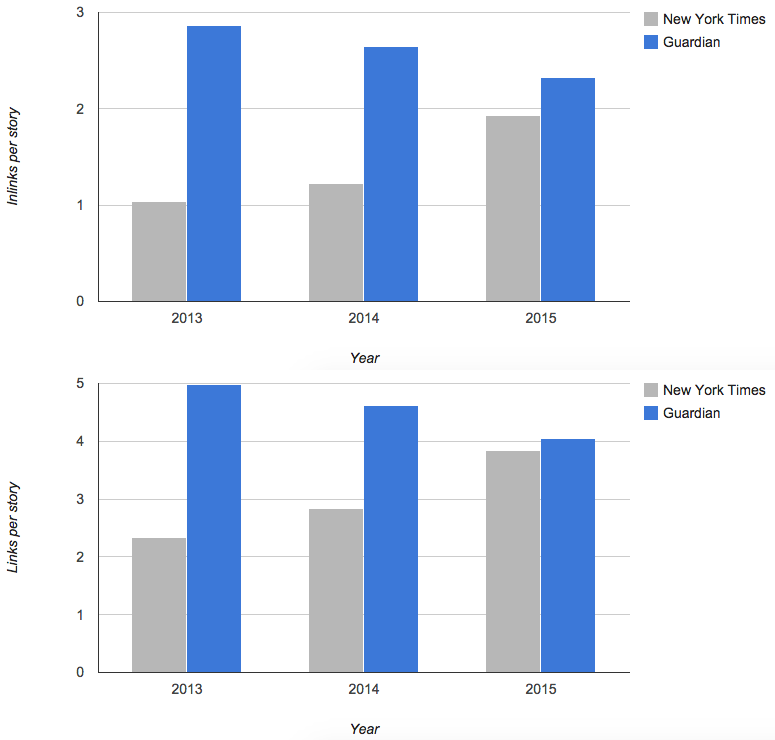
\includegraphics[width=400pt]{figures/nytvguardian-long}
\caption{New York Times and Guardian inline link data over time.}
\label{fig:nytvguardian-long}
\end{figure}

Finally, I broke each story into categories based on the category found in its URL. This allowed me to compare, first of all, whether linking practices changed radically across topics and desks; and second of all, whether certain topics were markedly different between the two publications. The Times' blogs stood out as the most often linked, but closer examination found that the increase was primarily due to outlinking. This would seem to reflect the institutional structure of the Times, as their blogs are intended to be somewhat free from the Times' usual approach, while adopting some of the spirit of online blogs. The Guardian's desks featured no similar pattern, but ranged from between 1 and 5 inlinks per story based on the desk.

While the Times and Guardian organize their content differently, I hoped to directly compare their practices across desks; as such, I manually merged the Times and Guardian data wherever overlaps between categories were apparent (for instance, each one had a \texttt{science} category and a \texttt{film} or \texttt{movies} category). In general, the Guardian featured consistently more links across desks, without great variation; however, some patterns emerged. Movies and theater were both relatively well-represented, suggesting that arts and culture content lends itself to linking. Each outlet's politics section likewise came out above average in inlinking. But some desks were noticeably below average for both, most strikingly their ``world'' sections, a topic that Tremayne suggested would require a great deal of context.

\begin{figure}[ht]
\centering
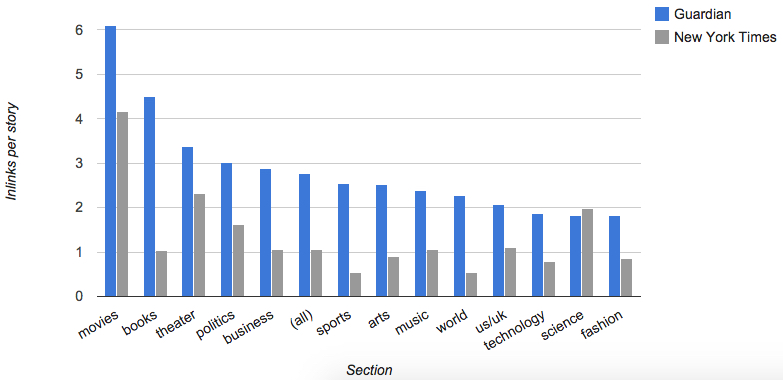
\includegraphics[width=450pt]{figures/nytvguardian-sections}
\caption{New York Times and Guardian inline link data by section.}
\label{fig:nytvguardian-sections}
\end{figure}

The third data set, gathered by crawling out from individual links to generate a network, was looking for linking deep into the past, or across traditional categories. I started with three incremental-update articles -- one each from the \emph{Times}, the \emph{Guardian}, and the \emph{Washington Post} -- about a single event: a March 2015 plane crash in the Alps. For each, the crawler generated a network; this resulted in a few dozen articles for the Guardian and the Post, but the Times crawler found thousands of articles and would have continued to crawl indefinitely. Visualizing the resulting networks, I found that the Guardian maintained the most robust network, more clustered than the Post's and featuring almost entirely relevant articles. For the Guardian, the crawler found a full 32 articles about the crash -- this is close to all of the relevant articles, and they self-organized through links without human intervention. However, the Post's articles dip farther back into the past, referencing articles about related plane crashes from decades earlier. These older articles benefit most from a link-oriented classification scheme, as they would otherwise need to be retroactively tagged in order to turn up as relevant, unless part of a complex hierarchy.

Tellingly, one day after running the Times' crawler (on March 27), I tried it again and found that the crawler stopped after gathering just three articles, rather than exploding into infinity. Looking into the article, I discovered that the article had been updated, and its crucial link removed. This points to the fragility of such a classification scheme unless reporters and editors are writing with links in mind. If the editor simply did not want to present such a link to the user, the editor could simply hide the link element in the text, making it invisible except to machines.

These results are preliminary, and more sample data is needed to determine how far a network-oriented scheme can work. Topic pages---or their modern equivalent, like Vox's card stacks---function as ``hubs'' that point to the stories themselves, the ``authorities.'' But authorities can be hubs on their own, measured by the quality of their links as much as their content; sometimes they link back to topic pages, and other times they link to one another. A link-oriented classification scheme might first need to establish the relationship between these new forms of hubs and authorities---and this relationship might be different for each publisher.

% directly to one another as well, and sometimes these direct links often help the deep, implicit archive emerge.
%But Vox provides a useful example of how a publication can build with link sustainability in mind. Their card stacks function like traditional topic pages, but because of the card-based orientation and Vox's focus on context, the links proliferate in interesting ways that begin to self-organize.

%Vox maintains just 1.8 inlinks per story, although they link out over 4 times as often. About 40\% of their stories Their stories cohere into a 

% Expand on Vox; then GET THIS SHIT DONE


% # April 2012
% # March 2013
% # February 2014
% # January 2015
% 	# Top 25 media (sample week?)
% 	# Top 1000 blogs (sample week?)

% # NYT
% # Guardian
% # Washington Post?

% # Time.com?
% # New Yorker?

% # Vox
% # Huffington Post
% # BuzzFeed? Gawker? FiveThirtyEight?

% # BBC
% # NPR
% # PBS

% # AP
% # Reuters

% Do stories with more links tend to be shorter? e.g. blogs?

% The last chapter dealt with how publishers think about their archives. This section focuses instead on how they're \emph{linking}, through research and quantitative link analysis. It will combine historic news network analyses and a study that I performed with the help of Media Cloud.

% This section will have quantitative analysis of inlinking vs. outlinking, both historical and my own research.
% Maybe call out 1-2 particular cases (NYT? Guardian? etc.) to see how they're linking


%Even once we assume that linking is a fundamental good for journalists, the problem remains of standardizing and developing a language \emph{for} linking, for this new affordance in citation and context provision.

% Anthony Grafton %  % Google books / Google scholar % % This should all probably be in a different place though %

%The digital realm, unbound by physical juxtapositions, can not only add an arbitrary number of links, but it can link \emph{in both directions}. Where paper books can only take a reader back in time, pointing only to its sources, it cannot tell you who used it as a source in turn. This results in what network scientists call a ``directed'' network, rather than a bidirectional one. to adds to these links.

% Jaron Lanier: "You're throwing away all the best parts of a network" (or Weinberger? Barabasi?). "Could not have greater implications"

% Adamic and others have tracked links across blogospheres and social networks. They rarely turn inward to a particular organization and see what they have to say.
% Deep examination of inlinks vs. outlinks. Usually Hyperlink Network Analysis specifically throws out the inlinks. So do search engines; called "nepotistic" links. This on the other hand hones in on them.
% Emphasize that I'm just using the content within the text of the article itself; there is much more. Anne Helmond "Exploring the Boundaries of a Website"; "The News Reads Us"

% More than this: Helmond MIT8 2013 -- New York Times pages have dozens of JavaScript trackers going, linked to other websites and services.

% Given these potentials, it might be surprising to find that many publishers are very reticent to link. Those who do have linking policies are often quite conservative.

% % OVERVIEW OF LINKING POLICIES: NYT, BBC, Guardian, etc. % % Reference to next section where I explain more what they're doing %

% Some of this is due to SEO; while no one knows exactly what Google's mercurial PageRank algorithm is doing, it's clear that links form a fundamental component (and as critics such as Clay Shirky have argued, relying on links rather than traditional categories and tags has been the crux of their success over competitors).\autocite{} Publishers are also wary of taking a reader away from their own website. But I'm also sure that much of the fear of links comes from inertia and tradition; since journalists never used to have a way to link, some don't see a need to start.

% While many have debated the potentials and pitfalls of hyperlinking the news, I am proposing an additional wrinkle to the conversation; a smart use of linking can be, to borrow Derrida's term, a \emph{pledge} to better structure the news and keep archives continuously animated and relevant.


% \section{Mapping Links}

% There is a lot of research on automatically mapping hyperlink networks; crawling, clustering, classifying utilizing a variety of machine learning techniques. However, most of these studies are interested in the ecosystem of content creators, and the ways in which links form across domains. My focus is instead on \emph{internal} links between stories. This is not only a more manageable set, but it is also allows opportunities for rich restructuring of the data schema. Chakrabarti says: "I believe that the Web will always remain adventurous enough that its most interesting and timely content can never be shoehorned into rigid schemata." This may be true, but internally, news publishers can use ankle-deep semantics to greatly improve their structures.

% Some webometrics endeavors have aimed to measure internal links within businesses, universities, etc. Others have done much work with internal clickstreams in order to gain insight about website usability. But nothing has looked at internal links of news stories.

% Some theory about how to do it. Talk to César? Reference De Maeyer's piece about it.
% Mapping, but also visualizing
% End by explaining my methodology

% De Maeyer "critical review of link studies". There are many limitations to webometrics. For instance, over-reliance on the information in the URL domain name and path, which we all agreed was not a uniform, consistent resource. This led to, e.g. Tuvalu being among the main hubs of developed countries in hyperlink network, because they sell their .tv domain.
% Maps of the blogosphere were popular in Web 2.0, they were "a link-driven genre" (De Maeyer 2013); but now we're in the era of platforms, how has that changed the link structure of the web?
% Also, a case against straight statistics and confidence intervals: "Links are not statistically independent observations, ‘because of factors such as imitation between web authors (…), the copying of pages or parts of pages, and automatic creation of web pages by server software’ (Thelwall, 2006: 7). According to Thelwall, this means that inferential statistics, such as confidence intervals, are not valid. As Harries et al. (2004) phrase it, web link creation is a ‘social activity that inspires imitation, the opposite of statistical independence’ (Harries et al., 2004: 439)."

% The goal, then: "semi-automatic methods". Most projects "rely on some manual coding, qualitative appreciations and human expertise." The main question is "when do we stop to purely describe the structure of links as technical objects and when do we start to relevantly exploit links to make sense of a social phenomenon?" But ultimately "mixed methods appropriately allow using hyperlinks as proxies for other phenomena." --  "combining quantitative link counts, qualitative inquiries and valuation of field expertise to support link interpretation."

% Fragoso 2011 tries to holistically combine the quantiative/qualitative, macro/micro study patterns that De Maeyer observes: "Web Science has favoured macroscopic approaches which have revealed much about the Web’s structural patterns. We argue that contextualised knowledge about hyperlinks on the Web has not advanced at the same rate and that complementary intermediate and micro-scale investigations are essential for a better understanding of the motivations, functions and meanings of these links."

% Could combine Media Cloud aggregate ``big data'' view with Times Newswire API (e.g. 1 month, ~9k stories) for deeper view into one publication. Deeper view could be a) anchor text, b) where the link is in relation to the top of the article, named entities, etc.

% \section{Automated NER and linked data potential}

% Can we get richer info automatically out of the entities referenced in newsrooms?

% Can we form networks out of the links that newspapers are making? Clusters, in network terms? How are they improvements on classifications, in a more traditional sense? a) they don't need to take as much account of the media type of the resource, right? Text, image, video, etc. are all treated semi-equally.

% Visualization of hyperlink networks: De Maeyer "Methods for Mapping Hyperlink Networks", Carriere/Kazman. De Maeyer "The web lacks geography," it's flat
% ``hyperlink maps are thus helpful in visualizing phenomena that would have been otherwise hard to detect: "the reason for performing such an analysis is to reveal latent structures that are not already obvious to an observer''


